\documentclass{beamer}

\usepackage[utf8]{inputenc}
\usepackage{hyperref}

\usetheme{Berkeley}
\beamertemplatenavigationsymbolsempty
\setbeamertemplate{headline}{}
 
\title{Geo-Visualisierung in FoodChain-Lab}
\date{}
 
\begin{document}
\maketitle

\section{Aufgaben}
\begin{frame}
	\begin{itemize}
		\item Nutzen Sie folgenden Workflow: \url{https://github.com/SiLeBAT/BfROpenLabResources/raw/master/GitHubPages/workflows/FCL_Example.zip}.
		\item Schauen Sie sich das Liefernetzwerk in der geographischen Ansicht vom \textbf{Tracing View} an.
		\item Selektieren Sie alle Stationen in Polen und schauen Sie sich dann an wo sich diese Stationen in der graphischen Ansicht befinden.
	\end{itemize}
\end{frame}
 
\section{1}
\begin{frame}
	\begin{center}
  		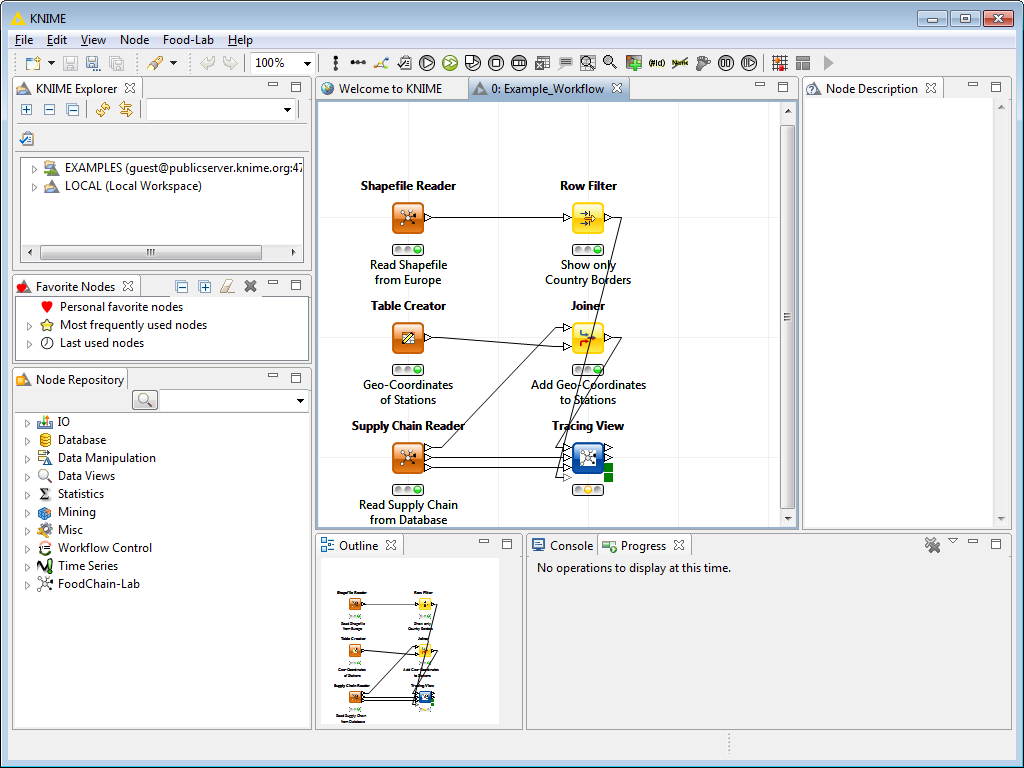
\includegraphics[height=0.6\textheight]{1.png}
	\end{center}
	\begin{itemize}
		\item Importieren Sie den Example Workflow von \url{https://github.com/SiLeBAT/BfROpenLabResources/raw/master/GitHubPages/workflows/FCL_Example.zip}.
		\item Öffnen Sie den \textbf{Tracing View} per Doppelklick.
	\end{itemize}
\end{frame}

\section{2}
\begin{frame}
	\begin{center}
  		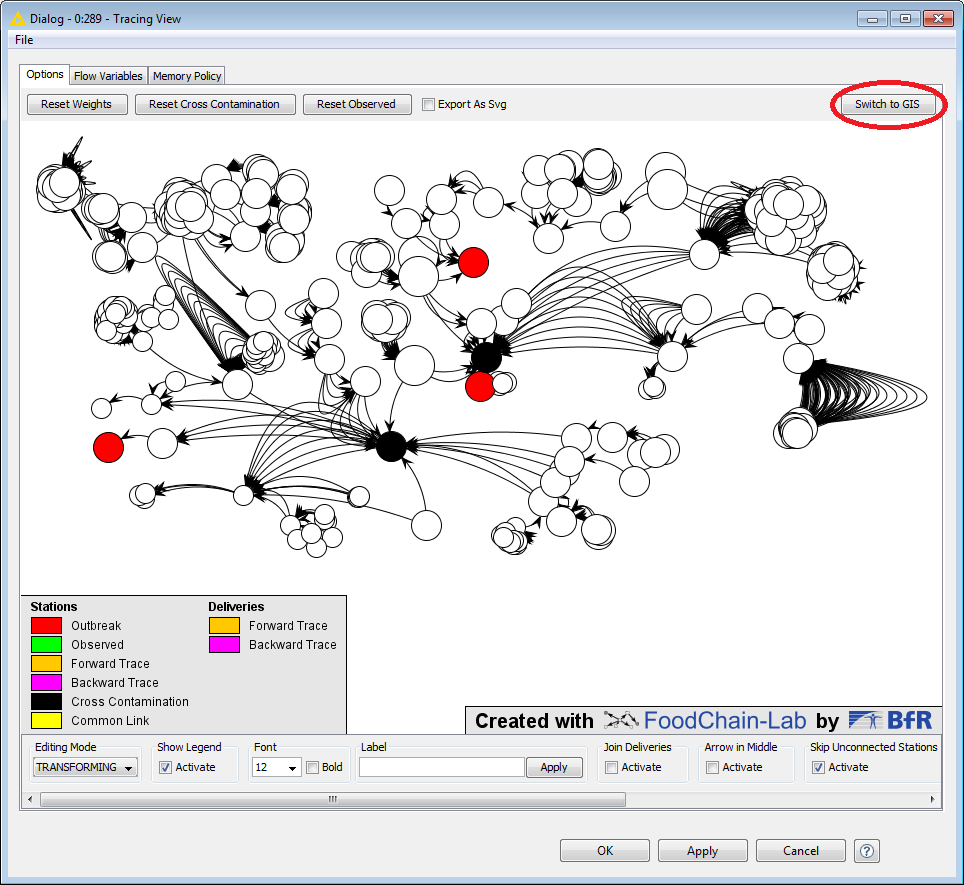
\includegraphics[height=0.6\textheight]{2.png}
	\end{center}
	\begin{itemize}
		\item Nun sehen Sie eine graphische Repräsentation des Liefernetzes.
		\item Um zur geographischen Repräsentation zu wechseln wählen Sie \textbf{Switch to GIS} rechts oben.
	\end{itemize}
\end{frame}

\section{3}
\begin{frame}
	\begin{center}
  		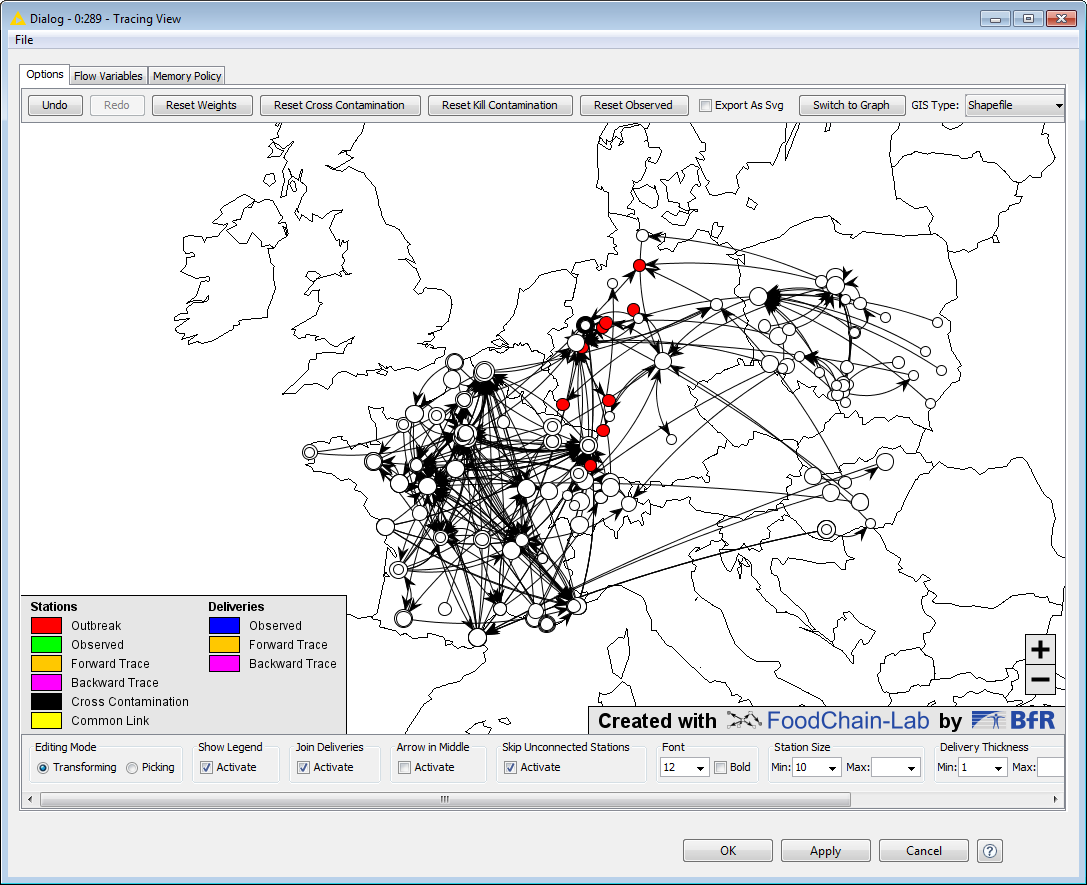
\includegraphics[height=0.6\textheight]{3.png}
	\end{center}
	\begin{itemize}
		\item Zur geographischen Visualisierung werden die Umrisse von Staaten genutzt, welche aus der Shapefile gelesen wurden.
		\item Um auf auf ein bestimmtes Gebiet zu zoomen wählen Sie "Transforming" als \textbf{Editing Mode} und nutzen Sie das Mausrad und die linke Maustaste zum Zoomen und Bewegen des Graphen (funktioniert wie in Google Maps).
	\end{itemize}
\end{frame}

\section{4}
\begin{frame}
	\begin{center}
  		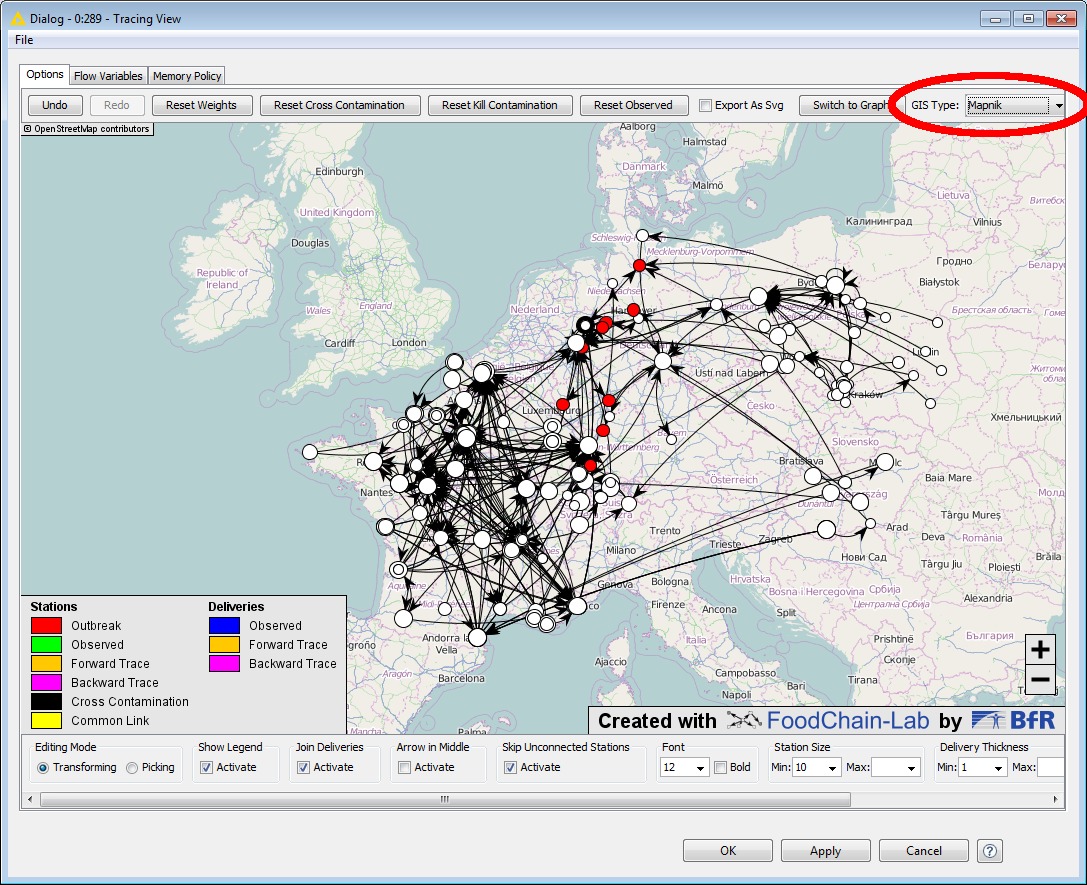
\includegraphics[height=0.6\textheight]{4.png}
	\end{center}
	\begin{itemize}
		\item Falls Sie mit dem Internet verbunden sind, können Sie die Art der Visualisierung ändern.
		\item Wählen Sie "Mapnik" als \textbf{GIS Type}.
		\item Nun sehen Sie eine Visualisierung mit OpenStreetMap Daten.
	\end{itemize}
\end{frame}

\section{5}
\begin{frame}
	\begin{center}
  		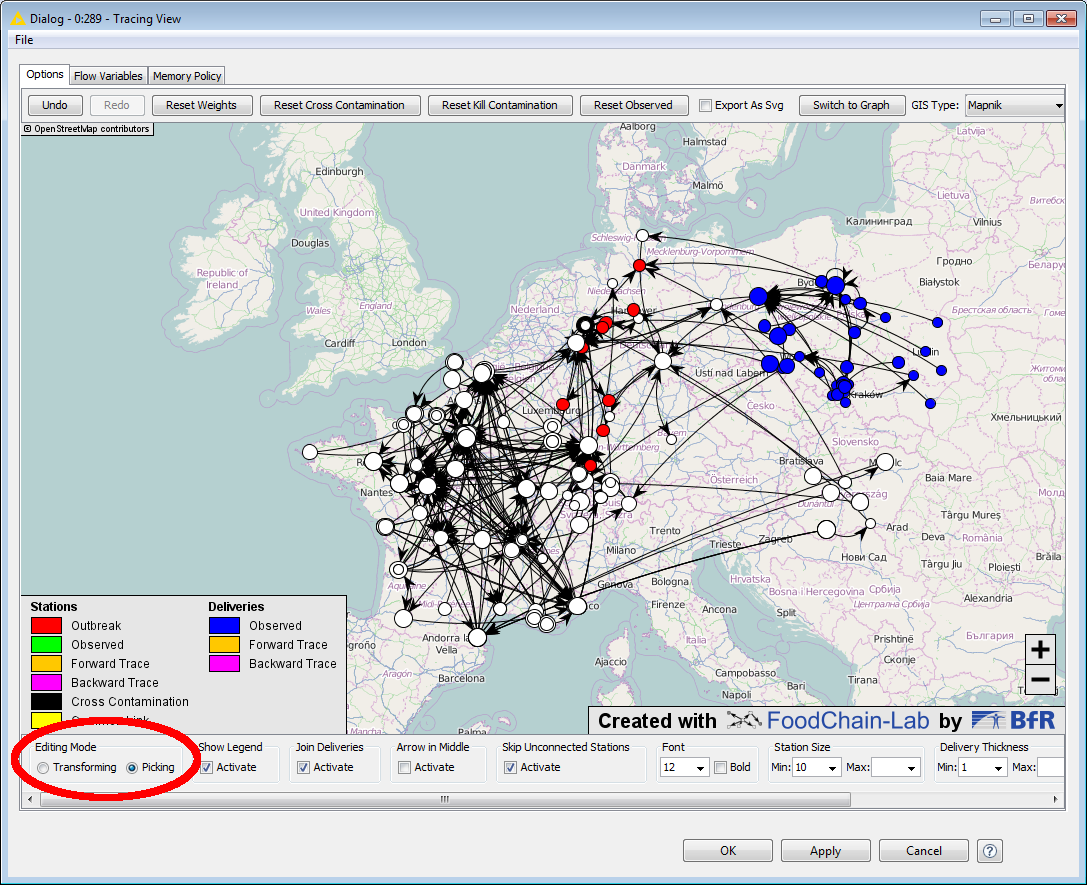
\includegraphics[height=0.5\textheight]{5.png}
	\end{center}
	\begin{itemize}
		\item Wir können nun Station aufgrund ihrer geographischen Lage auswählen.
		\item Setzen Sie "Picking" als \textbf{Editing Mode} and wählen Sie alle Stationen in Polen aus, indem Sie ein Rechteck um diese Stationen ziehen.
		\item The gewählten Stationen sollten nun blau markiert sein.
		\item Wechseln Sie zurück zur graphischen Ansicht, indem Sie rechts oben \textbf{Switch to Graph} klicken.
	\end{itemize}
\end{frame}

\section{6}
\begin{frame}
	\begin{center}
  		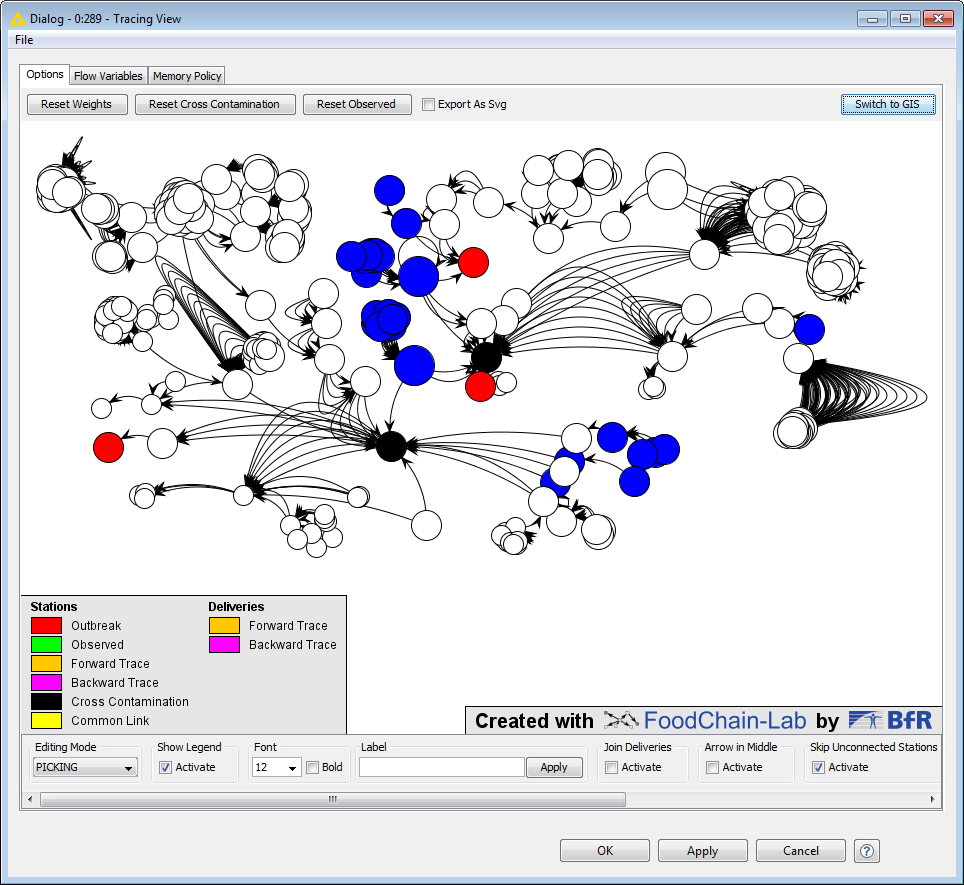
\includegraphics[height=0.5\textheight]{6.png}
	\end{center}
	\begin{itemize}
		\item Die blauen Stationen sind dieselben Stationen, die Sie in der geographischen Ansicht ausgewählt haben.
		\item Denn Änderungen, die Sie in einer Ansicht machen, werden automatisch auf die andere Ansicht übertragen.
		\item Das macht es einfach zwischen beiden Ansichten hin und her zu wechseln, um die Vorteile der jeweiligen Ansicht zu nutzen.
	\end{itemize}
\end{frame}

\section{7}
\begin{frame}
	\begin{center}
  		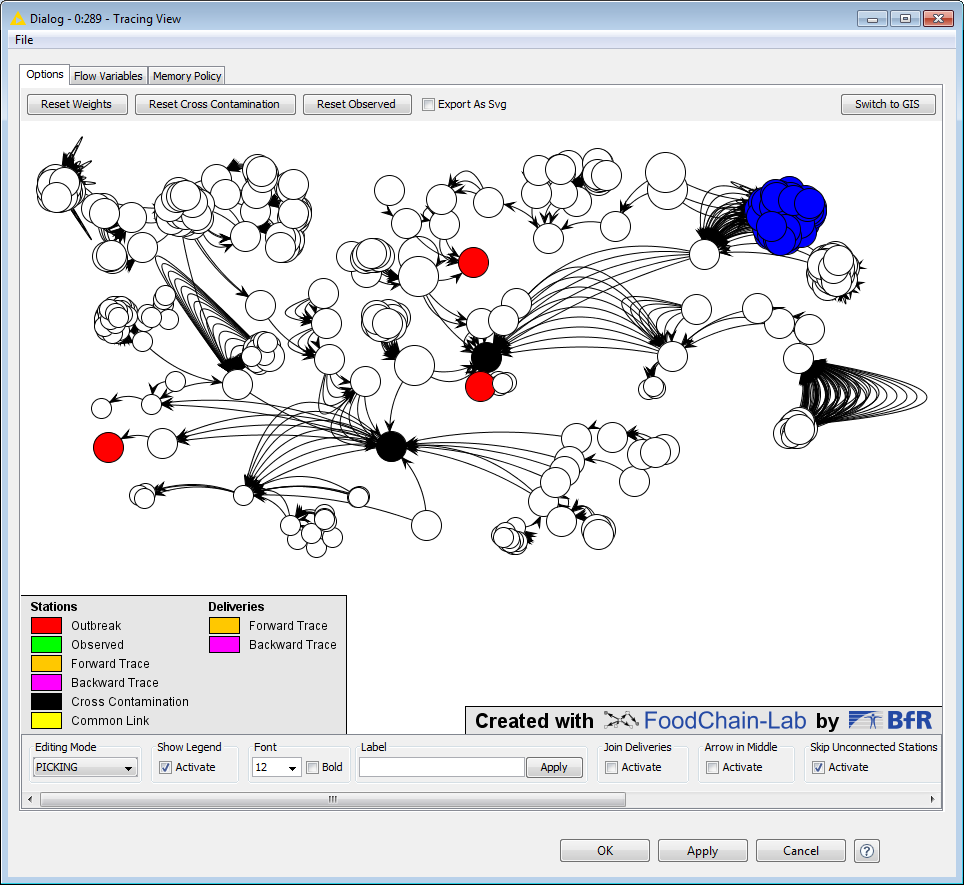
\includegraphics[height=0.6\textheight]{7.png}
	\end{center}
	\begin{itemize}
		\item Nun wählen wir ein "Cluster" von Stationen in der graphischen Ansicht und schauen uns dann die geographische Lage der Stationen an.
		\item Also wählen Sie das "Cluster" im roten Kreis und klicken Sie \textbf{Switch to GIS}.
	\end{itemize}
\end{frame}

\section{8}
\begin{frame}
	\begin{center}
  		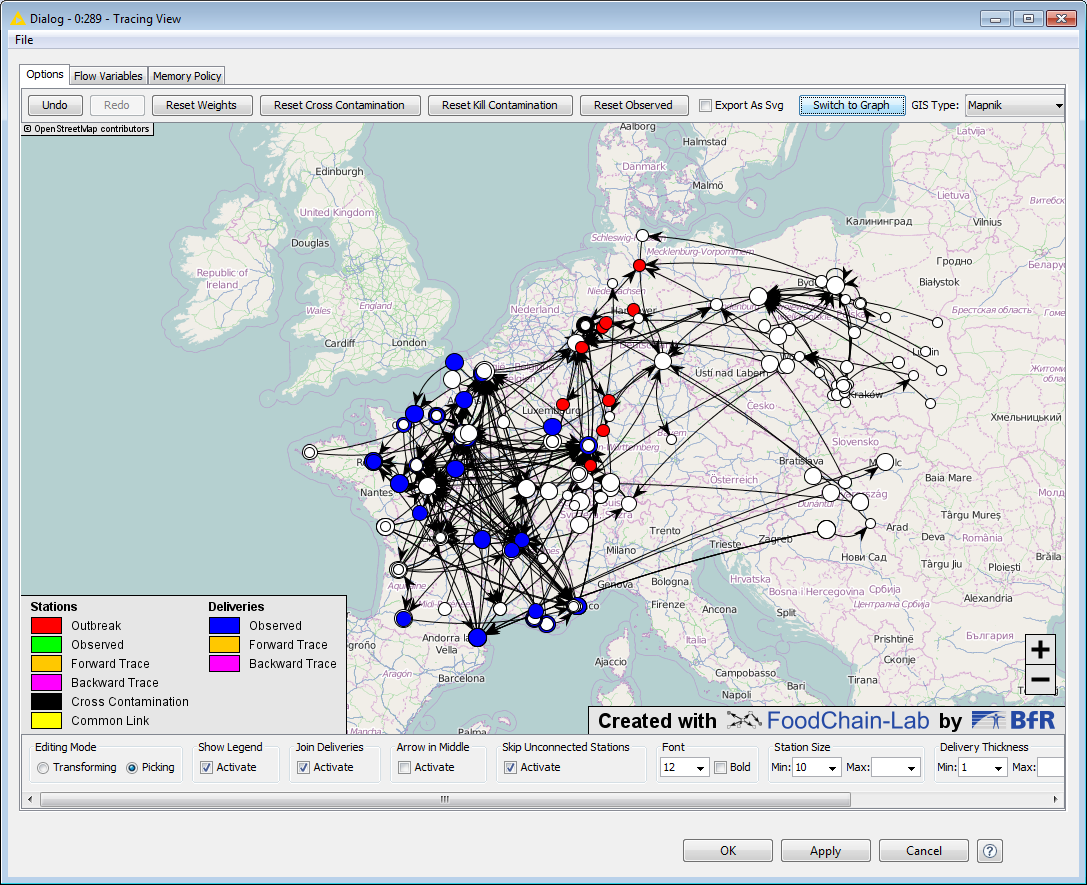
\includegraphics[height=0.6\textheight]{8.png}
	\end{center}
	\begin{itemize}
		\item Wie Sie sehen, sind die Stationen des Clusters über Frankreich verteilt.
	\end{itemize}
\end{frame}

\end{document}